\chapter{Basics of Wireless Communication}
\glsresetall
\label{chap:Wireless}

Wireless systems transmit data over the air using electromagnetic waves. These electromagnetic waves are converted to/from an electrical signal using an antenna. To transmit data, The antenna itself converts data encoded as an electrical signal into an electromagnetic wave which carries the information through the air. On the receive side, the antenna does the opposite; it converts the electromagnetic waves into a voltage across the antenna's terminals. 

The transmitted/received electrical signals are naturally real valued where the value represents the current provided to the antenna's terminals when transmitting or a voltage across the terminal when the systems is in receive mode. The signal can be varied over time in order to transmit information. The exact process used to convey this information is called the modulation. More specifically, modulation changes one or more properties of a high frequency signal which is called the \term{carrier signal}. This involves changing the signal's frequency, amplitude and/or phase. The carrier signal is at a much higher frequency than the data rate, e.g., WiFi uses 2.4 GHz.

Before we go any further on exactly how data is modulated, let us first provide some basic terminology. At its most simplistic form, a \term{signal} is something that conveys information. Mathematically, it is a function that maps a domain into a range. In the case of wireless communication, it is a mapping of time into a voltage or current. A \term{continuous signal} is a function defined of a continuous time interval.  A \term{discrete signal} has values defined at only certain points of time. A continuous signal can be converted into a discrete time signal by \term{sampling} where the \term{sampling interval} defines the time between two consecutive samples. The \term{sampling frequency} is the reciprocal of the sampling interval.  For example, a 1 GHz sampling frequency has a sampling interval of 1 ns. Wireless communication typically employs an \term{analog to digital converter (ADC)} to produce a discrete signal from the received continuous signal. This allows for digital processing of the signal in a general purpose microprocessor, digital signal processor, or FPGA, the latter of which is of course the focus of this book. A \term{digital to analog converter (DAC)} does the reverse; it converts a discrete signal into an continuous signal, e.g., to give to provide a current to the antenna to transmit a signal. 

\section{Modulation}
\label{subsec:modulation}

To convey information using a continuous carrier signal $A_c \cos (2 \pi f_c t + \phi)$, we can change the amplitude $A_c$, the phase $\phi$, and/or the frequency $f_c$. The basic techniques for the transmission of digital information include amplitude shift keying, phase shift keying, and frequency shift keying. Each of these techniques changes the specified portion of the signal in order to transmit a set of 'ones' and 'zeros'. The ``key'' is a discrete value encoded into the signal; in essence it is a transform between the digital (ones and zeros) to analog (carrier signal) domains. 

\begin{aside}
The term ``key'' is derived from Morse code key which is a device that turns something on or off. The straight key is probably the most familiar; it generates an electrical signal when the knob is pressed and is off otherwise.
\end{aside}

\term{Amplitude Shift Keying (ASK)} encodes data using the amplitude of the carrier signal. The simplest form of ASK is called \term{on-off keying} which uses the presence or absence of the carrier signal to represent a ``one'' or ``zero'', respectively. More generally speaking, ASK uses a finite number of amplitude to encode digital data, e.g., using four amplitudes would encode two binary bits.  \term{Phase Shift Keying (PSK)} uses the phase of the carrier signal to encode data. For example, the carrier's phase can be modulated between $0^{\circ}$ and $180^{\circ}$ in order to represent ``one'' and ``zero''. Additional phases can be used to encode more data, e.g., $0^{\circ}$, $90^{\circ}$, $180^{\circ}$, $270^{\circ}$ would represent two binary bits. \term{Frequency Shift Keying (FSK)} modulates the frequency in order to encode data. Binary FSK would use two different frequencies to encode ``zero'' and ``one''. Once again, additional frequencies can be used to encode more data.  Figure \ref{fig:keying} shows how four bits of binary data is encoded into the carrier signal using each of these modulation techniques.  \term{Quadrature Amplitude Modulation (QAM)} modulates both the amplitude and the phase. As such it can be viewed as simultaneously employing ASK and PSK to encode data.  

\begin{figure}
\centering
%\includesvg{keying}
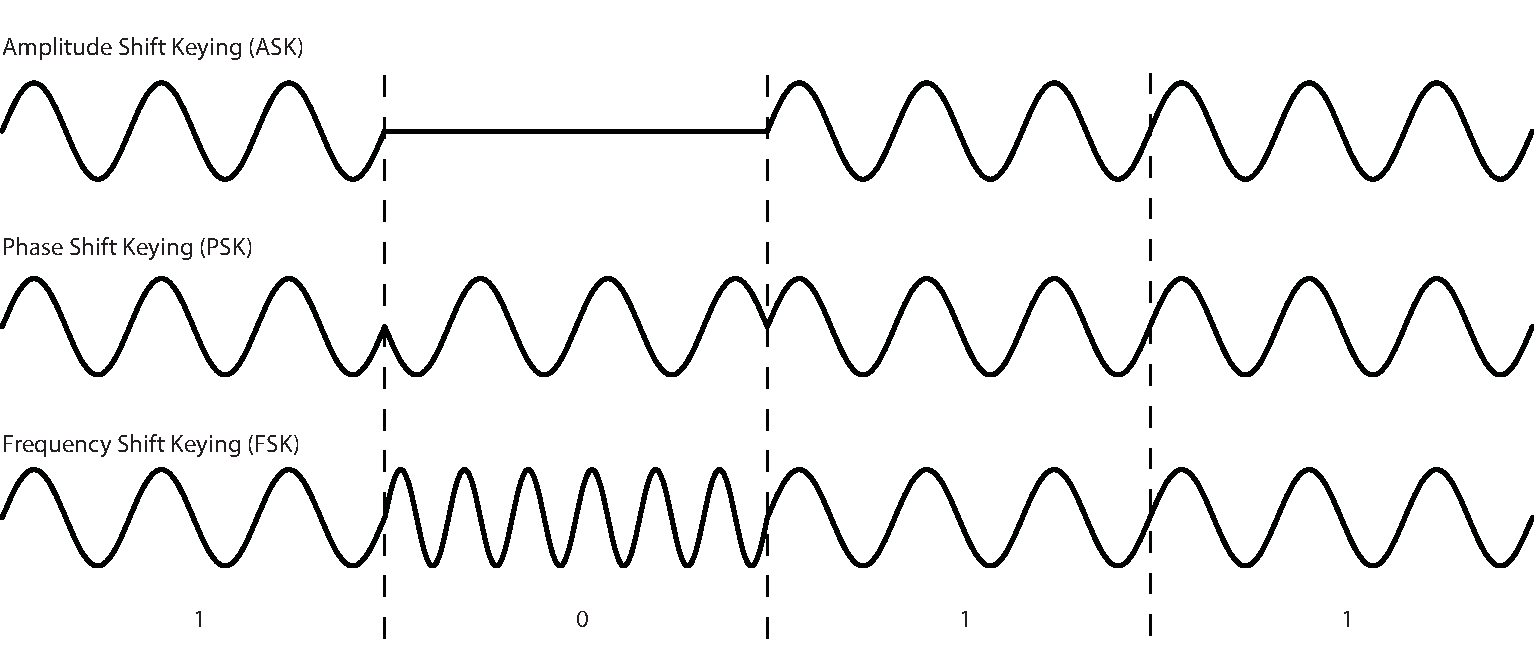
\includegraphics[width=.9\textwidth]{images/keying}
\caption{The ASK, PSK and FSK waveforms representing the binary data `1011'.}
\label{fig:keying}
\end{figure}

The job of the wireless receiver is to demodulate the received signal into a digital data. To do this, we must determine the key parameters of the carrier signal. Consider again the carrier signal $A_c \cos (2 \pi f_c t + \phi)$. Depending on the type of modulation, we need to extract the amplitude $A_c$, the frequency $f_c$, and/or the phase $\phi$. The frequency is the rate of change of the phase, i.e., $f_c$ is the first derivative of $\phi$ with respect to time ($f_c = \frac{\partial \phi}{\partial t}$). Therefore, if we know the amplitude $A_c$ and the phase $\phi$ at every instance of time, we can fully recreate the carrier signal. Because of this sinusoids are often represented using a polar coordinate system as in Figure \ref{fig:polar}. The amplitude of the sinusoid ($A_c$) is the length of the vector while the phase $\phi$ is the angle. The conversion between the polar and Cartesian coordinate system can be done using the trigonometric functions $x = A_c \cos \phi$ and $y = A_c \sin \phi$. The x axis is called the in-phase (I) or real axis portion of the signal while the y axis is called the quadrature (Q) or imaginary portion. 

\begin{figure}
\centering
%\includesvg{keying}
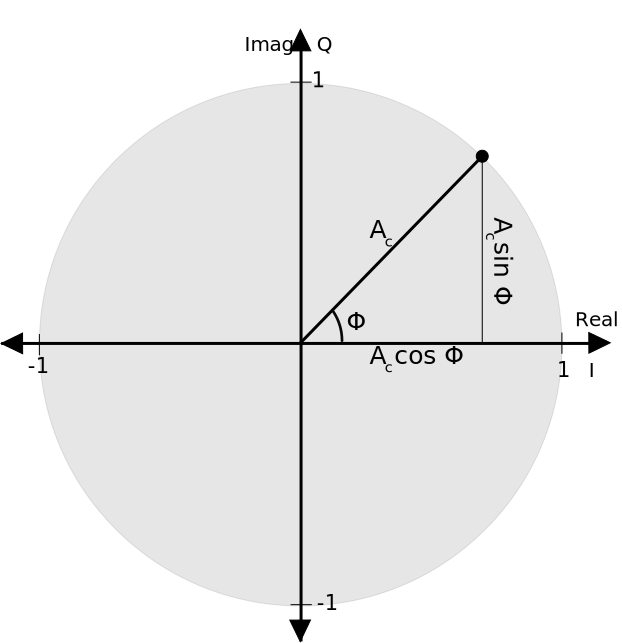
\includegraphics[width=.5\textwidth]{images/polar}
\caption{A polar coordinate representation of a sinusoid. The amplitude of the sinusoid is the length of the vector and the phase is the angle. The x axis is often referred to as the real or in-phase (I) value; similarly the y axis is the imaginary or quadrature (Q) value. }
\label{fig:polar}
\end{figure}

Since we modulate data based upon the amplitude, phase, and frequency, using polar coordinates is a natural way to represent and reasonable about wireless signals. Much of the mathematical foundations behind wireless communications utilize a polar representation. However, the discrete signal provided from/to the ADC and DAC is in terms of Cartesian coordinates, i.e., and I and Q or real and imaginary data. This is due to the fact that it is difficult (and therefore expensive) to change the phase of a high frequency carrier signal using an analog circuit. And it is relatively easy to create an analog circuit that varies the amplitude and phase of signal using I and Q data.

To do this, consider the following trigonometric identity:
\begin{equation}
\cos(u + v) = \cos(u) \cos(v) - \sin(u) \sin(v)
\end{equation}

If we transform the carrier signal using this identity we get:
\begin{equation}
A_c \cos (2 \pi f_c t + \phi) = A_c \cos (2 \pi f_c t) \cos(\phi) - A_c \sin (2 \pi f_c t) \sin(\phi)
\label{eq:carrier_identity}
\end{equation}

Noting that the real or in-phase (I) portion of the carrier signal at any instance of time is $A_c \cos \phi$ while the imaginary or quadrature portion is $y = A_c \sin \phi$ (see Figure \ref{fig:polar}), we can rewrite Equation \ref{eq:carrier_identity} as:

\begin{equation}
A_c \cos (2 \pi f_c t + \phi) = I \cos (2 \pi f_c t)  - Q \sin (2 \pi f_c t)
\end{equation}

The implications of this are that we can modulate the phase of the carrier signal by changing the amplitude of a sine and cosine wave of the same frequency. And therefore we can modify the amplitude, phase, and frequency of a carrier signal by changing the amplitude of a two signals of the same frequency separated by $-90^{\circ}$ phase offset. Or equivalently we can modulate the amplitude, phase, and frequency of a carrier signal using I and Q signals. It is much easier to create a circuit that performs this type of modulation as shown in Figure \ref{fig:IQcircuit}. The circuit requires two mixers (multipliers), a subtractor, and a phase change by $90^{\circ}$. Each of these components are relatively straightforward to design. As such, wireless data is very often represented as in-phase (I) and quadrature (Q).

\begin{figure}
\centering
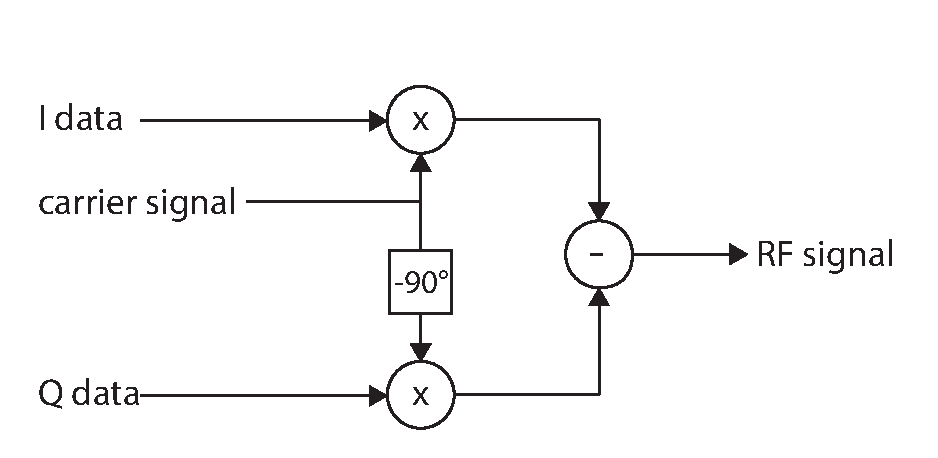
\includegraphics[width=.5\textwidth]{images/IQcircuit}
\caption{Circuit for generating an RF signal using I and Q data.}
\label{fig:IQcircuit}
\end{figure}

A basic understanding of I\textbackslash{}Q data and the complex plane allows for a better representation of the different modulation techniques. For example, we can denote binary PSK on the complex plane as shown in Figure \ref{fig:bpsk}. A carrier signal with a phase of $0^{\circ}$ encodes a value of `1' while a phase of $180^{\circ}$ denotes a value of `0'.  This is called a constellation diagram. This can be extended to more complex modulation techniques. For example, we can modulate data using both the amplitude and phase. This is called quadrature amplitude modulation (QAM), an example of which is shown in Figure \ref{fig:qam}. Here four bits are encoded into unique amplitudes and phases using a Gray code. The amplitude and phases are arranged into a rectangular fashion, which is common because they are easier to demodulate than other QAM constellations (e.g., circular). Note that BPSK can be considered as a special case of QAM, as can other ASK, PSK and FSK modulations. QAM is a popular modulation technique for higher data rate applications. For example, it is used in digital TV. 


\begin{figure}
\centering
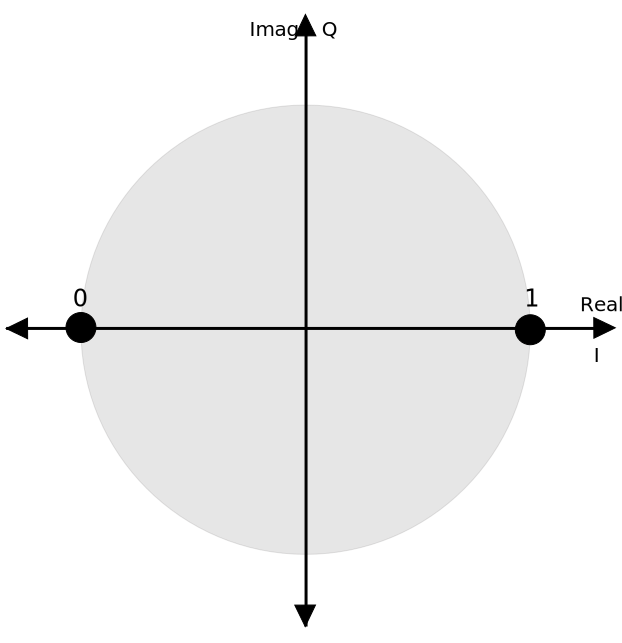
\includegraphics[width=.4\textwidth]{images/bpsk}
\caption{Binary Phase Shift Keying (BPSK) represented on the I\textbackslash{}Q plane using a constellation diagram.}
\label{fig:bpsk}
\end{figure}

\begin{figure}
\centering
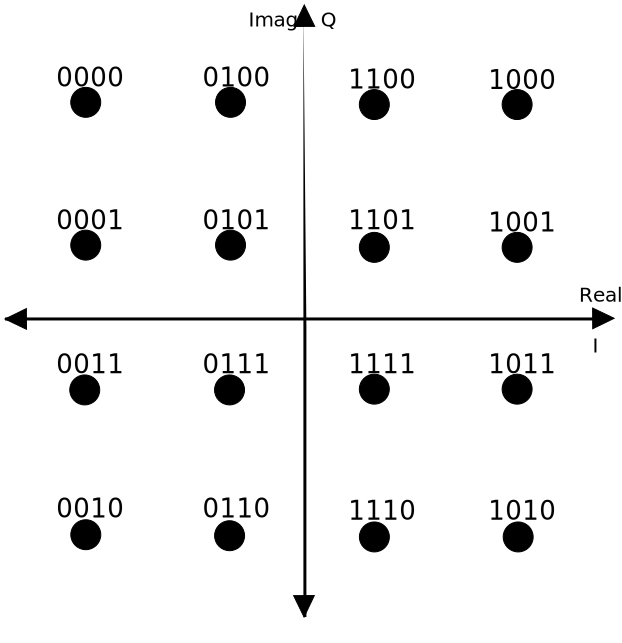
\includegraphics[width=.4\textwidth]{images/qam}
\caption{The constellation diagram of a 16 QAM modulation. Four bits are encoded using different phases and magnitudes across the  I\textbackslash{}Q plane.}
\label{fig:qam}
\end{figure}

\note{key relationship between matrices and complex numbers here:  This may help to define terminology from rotations in a 2D plane to complex numbers. Also this could be a series of asides relating these for readers that understand one side or the other. I think that keeping this as rotations and not bringing in complex numbers in this chapter is probably the right idea. } 


\note{I think remove the discussion of complex values and just focus on rotations in an x and y plane.}

\note{It might be useful to have an aside that shows the relationships between I, Q and phase and magnitude. Some formulas calculating with I/Q Signals translating between polar and rectangular form etc.
%Peak Amplitude A = (I?+Q?)?
%Phase Angle ? = tan??(Q/I)
%I = A?cos(?)
%Q = A?sin(?)
%Converting IQ Data to a plain signal: I is the original signal.
%Euler form: A?ei? = A?(cos(?) + i?sin(?)) = I + Qi
}

\note{Need to integrate this. It was moved from CORDIC which was rewritten.}

\note{Key idea: We very often want to view a signal in terms of frequency components. A frequency has an amplitude and phase. We often modulate data onto a signal using three components: amplitude, frequency and phase. Can talk about these three and give examples?}

\note{How does the ``complex'' come into this whole thing? Well through a magical formula called Euler's equation that relates sine and cosines to a complex exponential.}

\note{it is possible to encode information on a sine and cosine separately because they are orthogonal signals.}

\note{Negative frequencies: a ``crazy'' consequence of math? But actually show how there is more information when you consider the complex plane. A cosine can have both a positive and negative frequency. But this cannot be determined until you look at the orthogonal sine value (i.e., the ``imaginary'' portion). The negative frequency is a rotation in the ``opposite'' direction. 
}

Before we dive into the details, recall some basics of complex numbers. When multiplying two complex numbers, their phases add and their amplitudes (magnitudes) multiply. Consider two complex numbers
\begin{equation}
\begin{split} C_1 = I_1 + j \cdot Q_1 = A_1 (\cos \phi_1 + j \cdot \sin \phi_1)  \\
 C_2 = I_2 + j \cdot Q_2 = A_2 (\cos \phi_2 + j \cdot \sin \phi_2)
 \end{split}
\end{equation}
The first part of both equations is the complex number represented in Cartesian coordinates, where the real and imaginary parts are denoted as in-phase (I) and quadrature (Q) values. The second part is in polar form.  

Multiplying these two complex number yields
\begin{equation}
C_1 \cdot C_2 = (I_1 I_2 - Q_1 Q_2) + j \cdot (I_1  Q_2 + I_2  Q_1) = A_1 A_2 (\cos (\phi_1 + \phi_2) + j \cdot \sin(\phi_1 + \phi_2))
\label{eq:add_angle}
\end{equation}
You can see from the polar representation that the multiplication of these two complex numbers results in a summation of their phases (angles) and a multiplication of their amplitudes. Therefore, if we wish to rotate the complex number $C_1$ by some angle, we should multiply it by a second complex number $C_2$ that has a phase of that desired rotation angle. Going forward, we denote the rotating complex number as $C_R$. If we wish to subtract an angle, we can use the complex conjugate of $C_R$, i.e., ${C_R}^{*} = I_R - j \cdot Q_R$. Therefore to subtract the angle of complex number $C_R$ from $C_1$ we perform the complex multiplication
\begin{equation}
C_1 \cdot {C_R}^{*} = (I_1 I_R + Q_1 Q_R) + j \cdot (I_R  Q_1 - I_1  Q_R) = A_1 A_R (\cos (\phi_1 - \phi_R) + j \cdot \sin(\phi_1 - \phi_R))
\label{eq:sub_angle}
\end{equation}
Note the similarities between Equations \ref{eq:add_angle} and \ref{eq:sub_angle}. The major difference is that the signs are flipped in real and imaginary summations of the Cartesian multiply. This shows that the polar multiply performs addition and subtraction of the angles, respectively, as expected. An optimized CORDIC hardware design can take advantage of these similarities. 

\begin{aside}
Complex numbers are a useful representation for digital signal processing because they provide a simple way to model the phase and amplitude of a sinusoidal signal. For more information about this, please see Chapter \ref{subsec:modulation}. Most often in digital communications you will deal with complex numbers since it is easy to generate an analog to digital convertor that provides in-phase (real) and quadrature (complex) data. 

 An \term{imaginary number} was originally derived such that the roots of any polynomial equation, which are defined the solutions to any polynomial equation  
\begin{equation}
x^n + a_1 x^{n-1} + \cdots + a_{n-1} x + a_n
\label{eq:polynomial}
\end{equation}
such that the polynomial equation is equal to zero, i.e.,
\begin{equation}
x^n + a_1 x^{n-1} + \cdots + a_{n-1} x + a_n = 0.
\label{eq:poly_zero}
\end{equation}

Consider the polynomial $x^2 -1$, which we can factor as
\begin{equation}
x^2 - 1 = (x-1)(x+1).
\end{equation} This means the roots are $+1$ and $-1$. In general, if we can factor the polynomial in Equation \ref{eq:polynomial} as
\begin{equation}
x^n + a_1 x^{n-1} + \cdots + a_{n-1} x + a_n = (x - r_1)(x - r_2) \cdots (x - r_n),
\label{eq:poly_factor}
\end{equation} any value such that $x = r_i$ for any $i \in \{1, \cdots, n\}$ satisfies Equation \ref{eq:poly_zero}.

Now consider the polynomial $x^2 + 1$. This has no solution if we only consider real numbers. However, imaginary numbers provide a solution where the root is $\sqrt{-1} = j$. And with the introduction of imaginary numbers we can insure that every polynomial of degree $n$ can be factored into $n$ polynomials of degree one as demonstrated in Equation \ref{eq:poly_factor}.
\end{aside}

Once again, the CORDIC algorithm calculates various trigonometric functions through a set of rotations. First, consider rotating a complex number by $90^{\circ}$. To do this we multiply by $C_R = 0 + j$ since the phase of $C_R = 90^{\circ}$.  By substituting this into Equation \ref{eq:add_angle} and doing some simplification we get
\begin{equation}
C_1 \cdot C_R = - Q_1 + j \cdot I_1 = A_1 (\cos (\phi_1 + 90^{\circ}) + j \cdot \sin(\phi_1 + 90^{\circ}))
\label{eq:plus90}
\end{equation}
which is equivalent to negating the quadrature (imaginary) value of $C_1$ and swapping the in-phase (real) and quadrature values. Note that $A_R = 1$ and thus the amplitude complex number does not change with the rotation.  A similar effect occurs when we want to rotate $C_1$ by $-90^{\circ}$. In this case, we multiply by the complex number $C_R = 0 - j$ which gives us
\begin{equation}
C_1 \cdot C_R = Q_1 - j \cdot I_1  = A_1 (\cos (\phi_1 -  90^{\circ}) + j \cdot \sin(\phi_1 -  90^{\circ}))
\label{eq:minus90}
\end{equation}
which is equivalent to negating the in-phase value of $C_1$ and then swapping the in-phase and quadrature values. Thus, the computation for the rotation by $\pm 90^{\circ}$ is simply a negation and swapping of values which is simple and efficient in an FPGA.

Of course, we also need to efficiently rotate by values other than $90^{\circ}$. To do this, we perform rotations by multiplying by a complex number in the form of 
\begin{equation}
C_R = 1 + j \cdot 2^{-L}
\label{eq:complex_power2}
\end{equation} where $L = 0, 1, 2, 3, ... $ and thus the quadrature value $Q_R = 1, 0.5, 0.25, 0.125, ...$ . This probably seems like an odd choice but it will allow us to efficiently perform the complex multiplication. By substituting Equation \ref{eq:complex_power2} into Equation \ref{eq:add_angle} we get
\begin{equation}
C_1 \cdot C_R = (I_1 - Q_1 \cdot 2^{-L}) + j \cdot (I_1 \cdot 2^{-L} + Q_1) = (I_1 - Q_1 >> L) + j \cdot (I_1 >> L + Q_1)
\end{equation}

Note that calculating both the in-phase and quadrature values is done by a shift and add operation.  Additionally, if $L$ is a constant, then the shift can be implemented with wires in the FPGA, which has almost no resource cost. The rotation of the negative angle, which is done using the conjugate of $C_R$ provides a similarly efficient calculation with shifts and adds
\begin{equation}
C_1 \cdot C_R^{*} = (I_1 + Q_1 \cdot 2^{-L}) + j \cdot (Q_1 - I_1 \cdot 2^{-L}) = (I_1 + Q_1 >> L) + j \cdot (Q_1 - I_1 >> L)
\end{equation}

The next obvious question is what angle are we rotating by? And what about the amplitude of the resulting complex number after the rotation is performed? The phase of a complex number is calculated as 
\begin{equation}
\arctan (\frac{Q}{I})
\end{equation}
and the amplitude as
\begin{equation}
\sqrt{I^2 + Q^2}
\end{equation}
Thus the phase and amplitude of $C_R$ varies as shown in Table \ref{table:complexcordic}. The CORDIC gain is the running change in amplitude of the a complex number ($C_1$) who has gone through the sequential series of rotations of $C_R$ from $L = 0$ to the current value. Thus, the CORDIC gain when $L=0$ is simply the amplitude of $C_R$ when $L=0$, i.e., $| 1 + j | = 1.41421$. The CORDIC gain when $L = 1$ assumes that we have rotated by both $1 + j$, i.e., $C_R$ when $L=0$ and $1 + j \cdot 0.5$, i.e., $C_R$ when $L=1$. Thus the CORDIC gain is the amplitudes of these two $C_R$ numbers multiplied together, $1.41421 * 1.11803 = 1.58114$. You can see that as $L$ increases, the quadrature portion of $C_R$ starts to approach $0$. And as the angle gets smaller, the amplitude approaches $1$, and the CORDIC gain stabilizes to approximately 1.647. 

\note{make sure to look for references to table \ref{table:cordic} and change to \ref{table:complexcordic}.}

\begin{table}[htbp]
\caption{The phase, amplitude, and CORDIC gain of the rotating complex number $C_2$ as L varies.}
\begin{center}
\begin{tabular}{|c|c|c|c|c|c|}
\hline
L & $2^{-L}$ 	& $C_R$ 				& $C_R$ Phase ($^{\circ}$) 	& $| C_R |$ 		& CORDIC Gain 	\\ \hline \hline
0 & 1.0 		& $1 + j$  				& 45.000					& 1.41421			& 1.41421		\\ \hline
1 & 0.5 		& $1 + j \cdot 0.5$  		& 26.565					& 1.11803			& 1.58114		\\ \hline
2 & 0.25 		& $1 + j \cdot 0.25$  	& 14.036					& 1.03078			& 1.62980		\\ \hline
3 & 0.125 		& $1 + j \cdot 0.125$  	& 7.125					& 1.00778			& 1.64248		\\ \hline
4 & 0.0625 	& $1 + j \cdot 0.0625$  	& 3.576					& 1.00195			& 1.64569		\\ \hline
5 & 0.03125 	& $1 + j \cdot 0.03125$  	& 1.790					& 1.00049			& 1.64649		\\ \hline
6 & 0.015625 	& $1 + j \cdot 0.015625$  	& 0.895					& 1.00012			& 1.64669		\\ \hline
\end{tabular}
\end{center}
\label{table:complexcordic}
\end{table}%